\section{问题三：风格条件生成、感官画像与跨风格迁移}

问题三以细分风格标签为条件学习生成模型，在给定风格下生成化合物谱并给出感官画像，再把一种风格的化合物谱迁移为另一种风格，且缺陷化合物不恶化。
估计目标有三项：风格条件分布 $p(x\mid s)$、感官画像、以及满足两层缺陷约束的迁移映射。

\subsection{秩变换与风格条件潜在高斯模型}

图~\ref{fig:q3-flow} 给出问题三的完整流程。
风格和化学谱经秩变换与风格条件潜在高斯模型，经留出啤酒的保真、新颖性、可用性检查，得到感官画像与风味指纹，再经潜空间平移、化学投影、感官路径与原尺度复查完成迁移。

\begin{figure}[H]\centering
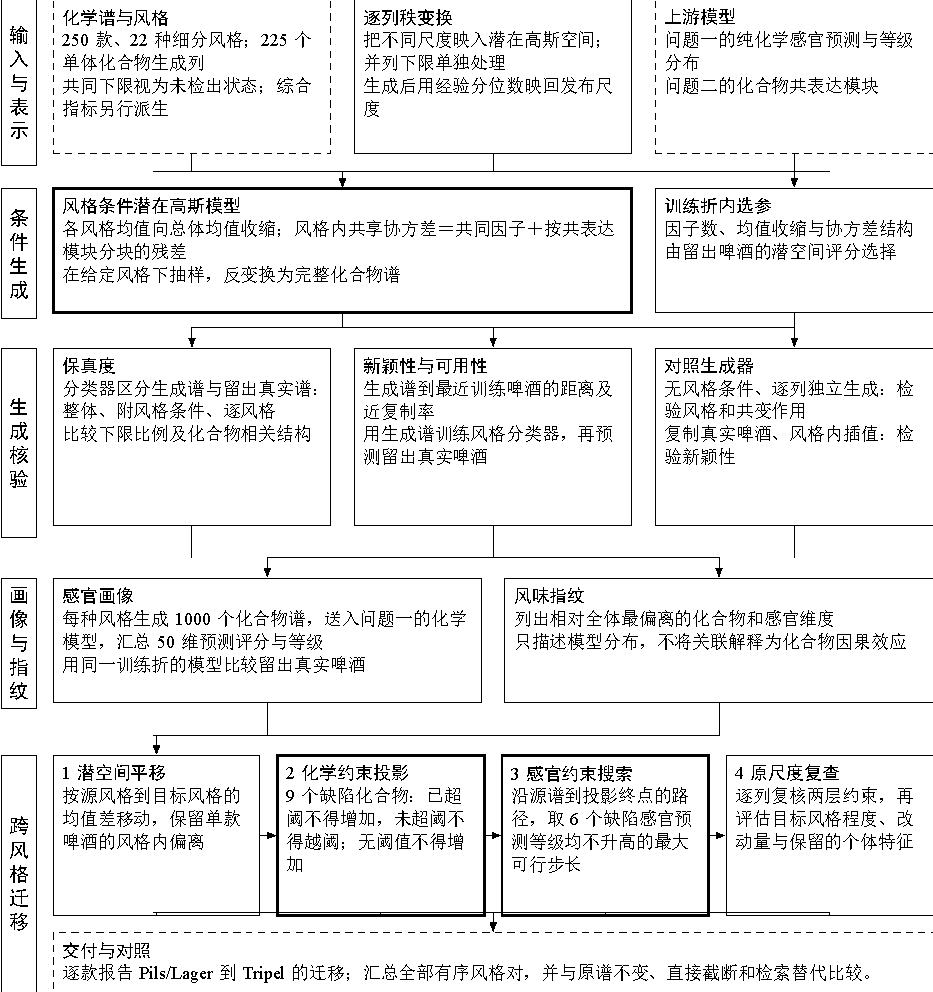
\includegraphics[width=\textwidth]{../figures/q3_methodology_flowchart.pdf}
\caption{问题三方法流程：风格和化学谱经秩变换与风格条件潜在高斯模型生成化合物谱，迁移经潜空间平移、化学投影、感官路径与原尺度复查。}
\label{fig:q3-flow}
\end{figure}

\subsubsection{并列下限的秩正态变换与经验分位数反变换}

生成器在逐列秩变换后的潜变量上建模。
对列 $j$ 取训练折的非缺失观测，把相同取值合并为块，块 $k$ 覆盖经验累积概率区间 $(l_k,h_k]$，块内所有观测的潜变量取标准正态在该区间上的条件期望：
\begin{equation}\label{eq:q3-rank}
\phi_j(x)=\mathbb E\!\left[Z\mid \Phi^{-1}(l_k)<Z\le\Phi^{-1}(h_k)\right]=\frac{\varphi(\Phi^{-1}(l_k))-\varphi(\Phi^{-1}(h_k))}{h_k-l_k} .
\end{equation}
式~\eqref{eq:q3-rank} 中 $\varphi$ 与 $\Phi$ 分别是标准正态的密度与分布函数。
无并列的取值时该式近似于正态得分，下限块的潜变量是截断正态的均值。
反变换 $x_j=Q_j(\Phi(u_j))$ 中 $Q_j$ 是保留并列取值全部概率质量的逆经验分布函数，把下限的整个概率区间映回下限值。

\subsubsection{风格均值收缩与因子模型加模块分块残差的协方差估计}

在潜空间中，同一风格内的潜变量服从多元正态分布：
\begin{equation}\label{eq:q3-gauss}
u_b\mid s(b)=s\ \sim\ \mathcal N(\mu_s,\ \Sigma_W),\qquad \Sigma_W=\Lambda\Lambda^\top+\Psi_M .
\end{equation}
式~\eqref{eq:q3-gauss} 中 $u_b$ 为啤酒 $b$ 的潜变量向量，$k$ 为因子数，$\Lambda$ 为 $225\times k$ 的因子载荷，$\Psi_M$ 为按问题二共表达模块分块的特异协方差。
风格均值向全局均值收缩：
\begin{equation}\label{eq:q3-shrink}
\hat\mu_s=\frac{n_s\bar u_s+\kappa\,\bar u}{n_s+\kappa},
\end{equation}
式~\eqref{eq:q3-shrink} 中 $n_s$ 为风格 $s$ 的啤酒数，$\bar u_s$ 为风格 $s$ 的样本均值，$\bar u$ 为全局均值，$\kappa$ 为收缩强度。
该式与问题一基线的收缩形式相同，小样本风格的均值估计由收缩稳定。
风格内协方差由合并风格内残差估计，先拟合因子载荷，再保留同一模块内的元素与对角元作为 $\Psi_M$，负特征值截到 $10^{-3}$ 保证正定。
各风格共享同一个 $\Sigma_W$，因为单个风格最多 31 款、少于 225 维，风格专属的完整协方差不可估计。

风格只解释每个化合物潜变量方差的一部分，风格解释的潜变量方差比例 $\eta^2$ 的中位数为 0.250，因此生成器必须同时刻画风格均值和风格内变化，只生成风格均值会丢掉约四分之三的方差。
风格内变化有低维结构，合并风格内残差的前 30 个主成分解释 72\% 的方差。
纯因子模型会衰减强相关的化合物对，模块块恢复这一共变，预运行中留出真实啤酒的模块内平均 Spearman 为 0.724，加模块块后生成样本为 0.680。

\subsection{生成模型选参与留出验证设计}

对生成结果提出三层合理性要求。取值层要求每列取值落在 250 款啤酒的观测范围内，未检出的下限作为离散状态按应有比例出现，综合指标与其成分一致。
分布层要求风格 $s$ 的生成样本与留出的风格 $s$ 真实啤酒在带风格标签的分类器双样本检验（C2ST，AUC 接近 0.5 表示未发现可区分性）中未表现出明显可区分性，也被独立的风格判别器判为 $s$。
新颖性要求生成样本不是训练啤酒的复制品。

生成器按风格分层、以单款啤酒为单位的 5 折交叉验证重复 5 次，种子 0 到 4；涉及感官标签的画像另用问题一的日期组外层划分，避免同一品评日期进入训练集与留出集两侧。
判别器与分类检验用随机森林 500 棵树、只用真实啤酒训练，与生成器不共享高斯假设；分类检验的置换 200 次并做真实对真实参照。
对照生成器五个：纯因子去掉模块块，无风格去掉风格条件，逐列独立去掉化合物间共变，复制直接复用训练啤酒，风格内插值在潜空间插值。
完整实验设置表与参数网格进附录。

选参在外层训练集内按留出潜空间评分完成，25 个外层折中有 24 折选因子加模块块、因子数 10、收缩强度 2，1 折选收缩强度 5；交付的全数据模型按同一规则选因子数 15、收缩强度 5。
下文的结果均以外层留出啤酒评价，选参不与报告复用同一划分。

\subsection{生成化合物谱及保真度、新颖性与可用性结果}

表~\ref{tab:q3-gen} 报告生成器验证的主要检验、对照与参照。
主模型在验收项 (a) 未通过：区分留出真实啤酒与生成样本的两样本分类检验，合并曲线下面积（AUC）为 0.589，条件曲线下面积为 0.576，均超出 $|\mathrm{AUC}-0.5|\le0.05$ 的预设标准，置换检验 $p$ 值为 0.017 与 0.032，真实对真实参照为 0.494 与 0.501，无风格对照为 0.642 与 0.634，逐列独立对照为 0.668，说明生成样本与真实啤酒仍可被区分，且这一差异来自下限状态共现而非检验偏差。
其余 (b) 到 (e) 通过：最近邻距离比 1.111，近复制率 0；在生成样本上训练的风格判别器识别留出真实啤酒的准确率为 0.481，真实对真实为 0.550；下限比例误差 0.021，复制参照为 0.014；模块内平均相关 0.667，真实留出为 0.724。
事后诊断把差异主要归于下限状态的共现：只用下限指示的分类检验 AUC 为 0.646，高于全谱的 0.564，生成样本中不同列同时未检出的程度约为真实的一半；其次是生成离散偏小，离散比为 1.17；把真实值截到训练范围后 AUC 不变，排除越界取值这一原因。

\begin{table}[H]
\centering\small
\caption{问题三生成器验证（占位，正式产物验收后填写）}
\label{tab:q3-gen}
\begin{tabular}{lcccccc}
\toprule
指标 & 主模型 & 纯因子 & 无风格 & 逐列独立 & 真实留出参照 & 验收阈值 \\
\midrule
取值层：下限比例误差 & 占位 & 占位 & 占位 & 占位 & 占位 & 占位 \\
取值层：每款下限列数 & 占位 & 占位 & 占位 & 占位 & 占位 & 占位 \\
分布层：合并 C2ST AUC & 占位 & 占位 & 占位 & 占位 & 占位 & 占位 \\
分布层：条件 C2ST AUC & 占位 & 占位 & 占位 & 占位 & 占位 & 占位 \\
分布层：风格内相关误差 & 占位 & 占位 & 占位 & 占位 & 占位 & 占位 \\
分布层：模块内相关 & 占位 & 占位 & 占位 & 占位 & 占位 & 占位 \\
新颖性：判别器距离比 & 占位 & 占位 & 占位 & 占位 & 占位 & 占位 \\
新颖性：近复制率 & 占位 & 占位 & 占位 & 占位 & 占位 & 占位 \\
\bottomrule
\end{tabular}
\end{table}

\subsection{基于评分预测分布的感官画像与风味指纹}

\subsubsection{生成谱的 50 维感官画像与留出参照}

感官画像由问题一的全数据模型给出。
对风格 $s$ 抽取 1,000 个潜变量样本，反变换得到化合物谱，经问题一模型得到 50 维连续预测与等级分布。
问题一主模型只用化学特征、不用风格，画像因此完全由生成的化合物谱决定。
问题一中化学模型未胜过风格基线的维度单独标注，这些维度上风格之间的画像差异不可靠。

图~\ref{fig:q3-portrait} 为三栏风格，行为 50 个维度，按六个维度组分块。
点与横线为生成画像的中位数及 10\% 到 90\% 区间，叠加同风格留出真实啤酒的折外预测中位数与观测均分中位数。
问题一未胜过风格基线的维度用灰色标签。

\begin{figure}[H]\centering
\fbox{\begin{minipage}[c][0.55\textwidth][c]{0.92\linewidth}
\centering\small 占位图：三栏感官画像，行为 50 个维度，点为生成画像中位数与区间，叠加真实啤酒的预测与观测。
出图后替换为 \texttt{\textbackslash includegraphics}。
\end{minipage}}
\caption{感官画像。三栏为三个风格，点与横线为生成画像的中位数与区间，叠加真实啤酒的预测与观测中位数。}
\label{fig:q3-portrait}
\end{figure}

画像验证在 16 个可评价风格上进行，生成器与问题一模型在同一外层训练集拟合，用同一感官模型分别预测生成谱与留出真实啤酒。
生成画像中位数与留出真实啤酒折外预测中位数的 Spearman 相关系数为 0.951，与留出观测均分的 Spearman 相关系数为 0.862，生成画像与留出观测均分的平均绝对差为 0.435 分。
生成画像 10\% 到 90\% 区间覆盖留出真实预测的比例为 0.720。
这些数值说明生成画像与同风格真实啤酒的预测基本一致，生成偏差与评分模型偏差被分开报告。

\subsubsection{化学偏移与感官差异的风味指纹}

风味指纹由化学指纹与感官指纹两部分组成。
化学指纹取标准化潜空间偏移 $\delta_{sj}=(\hat\mu_{sj}-\bar u_j)/\sqrt{\Sigma_{W,jj}}$，即该风格在化合物 $j$ 上偏离全体均值多少个风格内标准差，报告绝对偏移最大的 10 项。
感官指纹取画像中位数偏离全部风格合并画像中位数最大的维度。
化学解释在指纹产生后撰写，不改变指纹或模型。

图~\ref{fig:q3-fingerprint} 为三栏，分别为 Tripel、Kriek、Lambic。
每栏取化学指纹绝对偏移最大的 10 个化合物，同一模块只取一个。
每行一个化合物，箱线表示 1,000 个生成样本，散点表示该风格的真实啤酒，菱形与横线为化学指纹及其 bootstrap 区间。

\begin{figure}[H]\centering
\fbox{\begin{minipage}[c][0.55\textwidth][c]{0.92\linewidth}
\centering\small 占位图：三栏化学指纹，每栏取偏移最大的 10 个化合物，箱线为生成样本，散点为真实啤酒。
出图后替换为 \texttt{\textbackslash includegraphics}。
\end{minipage}}
\caption{化学指纹与生成谱。行名为化合物，箱线表示生成样本，散点表示真实啤酒，菱形为化学指纹及其区间。}
\label{fig:q3-fingerprint}
\end{figure}

\subsection{潜空间平移与缺陷约束下的跨风格迁移}

迁移任务以超阈值项界定缺陷，即化合物在阈值以下时不构成缺陷。
据此把不恶化写成两层约束。
化学层约束 9 个缺陷列，要求迁移后取值不高于上界，有阈值时上界为源取值与阈值中的较大者，无阈值时为源取值。
感官层约束 6 个缺陷维度，要求迁移后经问题一模型得到的预测等级不升高。
两层的比较对象都是迁移前的同一款啤酒，不是目标风格的典型值。

\subsubsection{风格均值差驱动的潜空间平移}

迁移映射是秩变换后的高斯近似下的潜空间平移，分四步执行。
第一步是平移。
在式~\eqref{eq:q3-gauss} 的模型下，协方差相同的两个高斯分布之间使潜空间代价最小的传输映射是平移：
\begin{equation}\label{eq:q3-shift}
\tilde u=u_b+\Delta_{s\to t},\qquad \tilde x_j=Q_j(\Phi(\tilde u_j)) .
\end{equation}
式~\eqref{eq:q3-shift} 中 $\Delta_{s\to t}=\hat\mu_t-\hat\mu_s$ 是目标风格与源风格的潜空间均值差，每款啤酒保留其相对本风格的个体偏离。

\subsubsection{化学缺陷上界下的马氏距离投影}

第二步是化学约束投影。
化学层约束换到潜空间后，$x'_j\le b_j$ 等价于 $u'_j\le\beta_j$。
求在潜空间马氏距离下最接近平移终点的可行点：
\begin{equation}\label{eq:q3-proj}
u^*=\arg\min_{u'}\ (u'-\tilde u)^\top\Sigma_W^{-1}(u'-\tilde u)\quad\text{满足}\quad u'_j\le\beta_j,\ j\in\mathcal D_c .
\end{equation}
约束只涉及 9 个坐标，用有效集法求解，其闭式解为 $u^*=\tilde u-\Sigma_{W,\cdot A}\,\Sigma_{W,AA}^{-1}(\tilde u_A-\beta_A)$，等于在缺陷坐标固定于上界时的条件均值。
缺陷化合物被压回上界时，与之共变的化合物按风格内协方差一起调整。
只截断缺陷列会产生数据中少见的组合，因此用投影而非截断。

\subsubsection{感官缺陷等级约束下的迁移强度搜索}

第三步是感官路径搜索。
感官层约束经问题一的树模型计算，不可微也不保证单调，不并入投影。
沿路径 $u(\alpha)=u_b+\alpha(u^*-u_b)$，$\alpha$ 从 0 到 1、步长 0.05，取满足感官约束的最大网格点 $\alpha^*$ 作为交付。
两端点都满足化学约束，可行集为凸集，整条路径满足化学约束。

\subsubsection{原尺度约束复查与缺失浓度的判断范围}

第四步是原尺度复查。
对交付的化合物谱在附件一原尺度逐列复查化学层上界，并用 231 列输入复查感官层。
复查不通过的候选视为不可行，$\alpha^*$ 取下一个可行网格点。

\subsection{Pils/Lager 向 Tripel 迁移结果与跨风格汇总}

表~\ref{tab:q3-transfer} 为 Pils/Lager 到 Tripel 的 11 款逐款结果，列为啤酒、迁移强度、源谱与交付谱的目标风格概率、结论类别、起作用的化学约束数、首个不可行点违反的感官维度、原尺度改变列数与保留度。
图~\ref{fig:q3-transfer-fig} 两栏对应此表，左栏为各方法的 Tripel 概率，右栏为 11 乘 15 的约束矩阵，直接证明缺陷不恶化。

\begin{table}[H]
\centering\small
\caption{Pils/Lager 到 Tripel 逐款迁移（占位，正式产物验收后填写）}
\label{tab:q3-transfer}
\begin{tabular}{lccccccc}
\toprule
啤酒 & $\alpha^*$ & 源谱 $P$(Tripel) & 交付谱 $P$(Tripel) & 结论类别 & 化学约束数 & 违反维度 & 保留度 \\
\midrule
占位 & 占位 & 占位 & 占位 & 占位 & 占位 & 占位 & 占位 \\
\bottomrule
\end{tabular}
\end{table}

\begin{figure}[H]\centering
\fbox{\begin{minipage}[c][0.55\textwidth][c]{0.92\linewidth}
\centering\small 占位图：左栏为各方法的目标风格概率，右栏为 11 乘 15 约束矩阵。
出图后替换为 \texttt{\textbackslash includegraphics}。
\end{minipage}}
\caption{迁移的代价与收益。左栏为各方法的 Tripel 概率，右栏为化学与感官约束矩阵，直接证明缺陷不恶化。}
\label{fig:q3-transfer-fig}
\end{figure}

图~\ref{fig:q3-pairs} 为 22 乘 22 热图，格内颜色为源风格啤酒达到参照范围的比例，对角留空，行列按风格潜空间均值的层次聚类排序，行尾附平均迁移强度的条形边栏。

\begin{figure}[H]\centering
\fbox{\begin{minipage}[c][0.55\textwidth][c]{0.92\linewidth}
\centering\small 占位图：22 乘 22 风格对热图，格内为源风格啤酒达到参照范围的比例，行尾为平均迁移强度。
出图后替换为 \texttt{\textbackslash includegraphics}。
\end{minipage}}
\caption{风格对热图。行列按风格潜空间均值的层次聚类排序，图注写明风格对之间不独立。}
\label{fig:q3-pairs}
\end{figure}

Pils/Lager 向 Tripel 迁移的 11 款啤酒中，最大可行迁移强度 $\alpha^*$ 的中位数为 1.0，8 款达到投影终点，无一款退回 0。
源谱的 Tripel 判别概率中位数为 0.046，交付谱提高到 0.164，真实 Tripel 啤酒的交叉拟合概率中位数为 0.269。
按预先固定的四类结论，7 款达到参照范围、2 款改善、2 款未改善，其中 2 款因双乙酰浓度缺失只能在填补设定下判断。
原尺度复查下化学层与感官层违约数均为 0，平移不施加约束时 11 款全部违反化学层约束。
462 个有序风格对中，平移后至少违反一项化学约束的啤酒比例中位数为 1.0，施加两层约束后约束起作用比例的中位数为 0.890，迁移后目标风格概率中位数为 0.092。
迁移只沿一条线段搜索，迁移强度小只说明该路径受限，不说明不存在满足约束的目标风格化合物谱。

\subsection{协方差结构、风格差异与缺陷约束的敏感性分析}

敏感性分析每次只改动一个环节，其余保持主设定，报告基线值、改动值及逐次配对差的 95\% 区间。
生成侧，去掉模块块改用纯因子或 Ledoit--Wolf 收缩主要降低模块内平均相关，配对差分别为 $-0.036$ 与 $-0.065$，合并分类检验曲线下面积的变化区间含 0 或接近 0，其余指标基本不变。
收缩强度向上移一格使合并曲线下面积升至 0.680，向下移一格降至 0.549，说明该检验对收缩强度敏感，但这是外层评价结果，只报告，不改选主模型。
风格离散比超过 1.5 的风格只有 Brut，其余风格未推翻共享协方差的假设。
迁移侧，化学层改用严格不增加规则后约束起作用比例由 0.853 升至 0.969，11 款交付谱的 Tripel 概率中位数由 0.164 降至 0.128。
感官层改用连续预测不升高时，迁移强度中位数由 1.0 降至 0，说明感官层约束主要由预测等级规则承载。
问题一映射改用分位数切点等级时迁移强度中位数由 1.0 降至 0.9。
主要结论在协方差结构、缺失处理、附件取值与阈值口径下保持稳定，完整的臂间结果进附录。
